\documentclass[border=5pt]{standalone}
\usepackage[T1]{fontenc}
\usepackage{lmodern,amsmath,amssymb,mathtools,tikz,tikz-cd}
\usetikzlibrary{arrows.meta,positioning,calc,decorations.markings}
\newcommand{\C}{\mathbb C}\newcommand{\R}{\mathbb R}\newcommand{\Z}{\mathbb Z}
\newcommand{\gshift}[2]{#1\langle #2\rangle}
\begin{document}
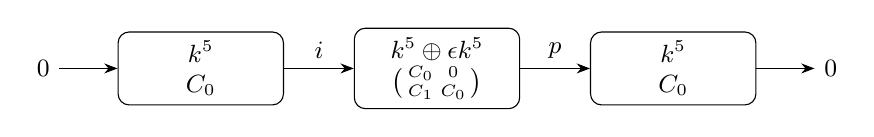
\begin{tikzpicture}[>=Stealth,every node/.style={font=\small},
 box/.style={draw,rounded corners,align=center,minimum width=2.1cm,minimum height=.9cm}]
\node (z) at (0,0) {$0$};
\node[box] (l) at (2,0) {$k^5$\\$C_0$};
\node[box] (m) at (5,0) {$k^5\oplus\epsilon k^5$\\$\left(\begin{smallmatrix}C_0&0\\C_1&C_0\end{smallmatrix}\right)$};
\node[box] (r) at (8,0) {$k^5$\\$C_0$};
\node (e) at (10,0) {$0$};
\draw[->] (z)--(l);\draw[->] (l)--node[above] {$i$}(m);
\draw[->] (m)--node[above] {$p$}(r);\draw[->] (r)--(e);
\end{tikzpicture}
\end{document}
